% Options for packages loaded elsewhere
\PassOptionsToPackage{unicode}{hyperref}
\PassOptionsToPackage{hyphens}{url}
\PassOptionsToPackage{dvipsnames,svgnames*,x11names*}{xcolor}
%
\documentclass[
  10pt,
  ignorenonframetext,
  table, dvipsname, compress]{beamer}
\usepackage{pgfpages}
\setbeamertemplate{caption}[numbered]
\setbeamertemplate{caption label separator}{: }
\setbeamercolor{caption name}{fg=normal text.fg}
\beamertemplatenavigationsymbolsempty
% Prevent slide breaks in the middle of a paragraph
\widowpenalties 1 10000
\raggedbottom
\setbeamertemplate{part page}{
  \centering
  \begin{beamercolorbox}[sep=16pt,center]{part title}
    \usebeamerfont{part title}\insertpart\par
  \end{beamercolorbox}
}
\setbeamertemplate{section page}{
  \centering
  \begin{beamercolorbox}[sep=12pt,center]{part title}
    \usebeamerfont{section title}\insertsection\par
  \end{beamercolorbox}
}
\setbeamertemplate{subsection page}{
  \centering
  \begin{beamercolorbox}[sep=8pt,center]{part title}
    \usebeamerfont{subsection title}\insertsubsection\par
  \end{beamercolorbox}
}
\AtBeginPart{
  \frame{\partpage}
}
\AtBeginSection{
  \ifbibliography
  \else
    \frame{\sectionpage}
  \fi
}
\AtBeginSubsection{
  \frame{\subsectionpage}
}
\usepackage{lmodern}
\usepackage{amsmath}
\usepackage{ifxetex,ifluatex}
\ifnum 0\ifxetex 1\fi\ifluatex 1\fi=0 % if pdftex
  \usepackage[T1]{fontenc}
  \usepackage[utf8]{inputenc}
  \usepackage{textcomp} % provide euro and other symbols
  \usepackage{amssymb}
\else % if luatex or xetex
  \usepackage{unicode-math}
  \defaultfontfeatures{Scale=MatchLowercase}
  \defaultfontfeatures[\rmfamily]{Ligatures=TeX,Scale=1}
\fi
% Use upquote if available, for straight quotes in verbatim environments
\IfFileExists{upquote.sty}{\usepackage{upquote}}{}
\IfFileExists{microtype.sty}{% use microtype if available
  \usepackage[]{microtype}
  \UseMicrotypeSet[protrusion]{basicmath} % disable protrusion for tt fonts
}{}
\makeatletter
\@ifundefined{KOMAClassName}{% if non-KOMA class
  \IfFileExists{parskip.sty}{%
    \usepackage{parskip}
  }{% else
    \setlength{\parindent}{0pt}
    \setlength{\parskip}{6pt plus 2pt minus 1pt}}
}{% if KOMA class
  \KOMAoptions{parskip=half}}
\makeatother
\usepackage{xcolor}
\IfFileExists{xurl.sty}{\usepackage{xurl}}{} % add URL line breaks if available
\IfFileExists{bookmark.sty}{\usepackage{bookmark}}{\usepackage{hyperref}}
\hypersetup{
  colorlinks=true,
  linkcolor=Black,
  filecolor=Maroon,
  citecolor=Blue,
  urlcolor=Maroon,
  pdfcreator={LaTeX via pandoc}}
\urlstyle{same} % disable monospaced font for URLs
\newif\ifbibliography
\setlength{\emergencystretch}{3em} % prevent overfull lines
\providecommand{\tightlist}{%
  \setlength{\itemsep}{0pt}\setlength{\parskip}{0pt}}
\setcounter{secnumdepth}{-\maxdimen} % remove section numbering
%\usepackage{pslatex} % to see correctly a .pdf file on the computer screen
\usepackage{pgf}
\usepackage{color}
\usepackage{graphicx}
\usepackage{amssymb} %symbole de maths
\usepackage{amsmath} %idem
\usepackage[utf8]{inputenc}
%\usepackage{fancyvrb} %give size to verbatim
%\usepackage{hyperref}
\usepackage[english,francais]{babel}
\definecolor{vertmoyen}{RGB}{51,110,23} % vert moyen
\definecolor{blueFRB}{HTML}{31859c}
\usecolortheme[named=blueFRB]{structure}
\usepackage{tabularx} % varier la largeur du tableau
\usepackage{layout}
\usepackage{longtable}
\setlength{\LTleft}{-5cm plus 1 fill}
\setlength{\LTright}{-5cm plus 1 fill}
\usepackage{booktabs}
\usepackage{arydshln} %% dashlines for tabular
\newcommand{\logit}{\text{logit}}
\newcommand{\bs}[1]{\boldsymbol{#1}}
\newcommand{\R}{\textnormal{\sffamily\bfseries R}}
\newcommand{\pkg}[1]{{\fontseries{b}\selectfont #1}}
\newcolumntype{C}[1]{>{\centering\arraybackslash}m{#1}}
%% Natbib is a popular style for formatting references.
%\usepackage{natbib} %doesn't work with beamer

\title[JSDM-Metradica]{Assessing tree species vulnerability to climate change in French Guiana using joint species distribution models}
%\subtitle{} 

\author{}
\date{\vspace{-2.5em}}

% Theme
% \usetheme{AnnArbor}
% \usetheme{Dresden}
% \usetheme{Copenhagen}
% \usetheme{Frankfurt}
% \usetheme{Berlin}
% \usetheme{Madrid}
% \usetheme{Montpellier}
% \usetheme{Singapore}
% \usetheme{Antibes}
\useinnertheme{rounded} %% bullets
\useoutertheme[subsection=false]{miniframes}
\setbeamertemplate{footline}[frame number]
\setbeamertemplate{frametitle}{%
    \usebeamerfont{frametitle}\insertframetitle%
    \vphantom{g} % To avoid fluctuations per frame
    \par
    \centering 
\includegraphics[width=\textwidth]{figs/Barre_couleur}
}

% Ignore ignorenonframetext class option in default template
\makeatletter
\beamer@ignorenonframefalse
\makeatother

% Logo
\newif\ifplacelogo % create a new conditional
\logo{\ifplacelogo
\includegraphics[width=0.5\textwidth]{figs/partners_logos}\fi} % replace with your own command

%Call table of contents at the beginning of each section
\AtBeginSection[]{
\placelogotrue
  \begin{frame}
    \frametitle{Plan}
    \begin{columns}[c]
      \begin{column}{0.5\textwidth}
        \tableofcontents[sections=1,currentsection]
        \vspace{0.5cm}
        \tableofcontents[sections=2,currentsection]
      \end{column}
      \begin{column}{0.5\textwidth}
        \tableofcontents[sections=3,currentsection]
        \vspace{0.5cm}
        \tableofcontents[sections=4,currentsection]
      \end{column}
    \end{columns}
  \end{frame}
\placelogofalse
}

\AtBeginSubsection[]{}

% \AtBeginSubsection[]{
% \placelogotrue
%   \begin{frame}
%     \frametitle{Plan}
%     \begin{columns}[c]
%       \begin{column}{0.5\textwidth}
%         \tableofcontents[sections={1-2},currentsection,currentsubsection]
%       \end{column}
%       \begin{column}{0.5\textwidth}
%         \tableofcontents[sections={3-4},currentsection,currentsubsection]
%       \end{column}
%     \end{columns}
%   \end{frame}
% \placelogofalse  
% }

% Two-columns slides
\def\bcols{\begin{columns}}
\def\bcol{\begin{column}}
\def\ecol{\end{column}}
\def\ecols{\end{columns}}
\ifluatex
  \usepackage{selnolig}  % disable illegal ligatures
\fi

\author{}
\date{}

\begin{document}

% {
%   % Use background image
%   \usebackgroundtemplate{%
%     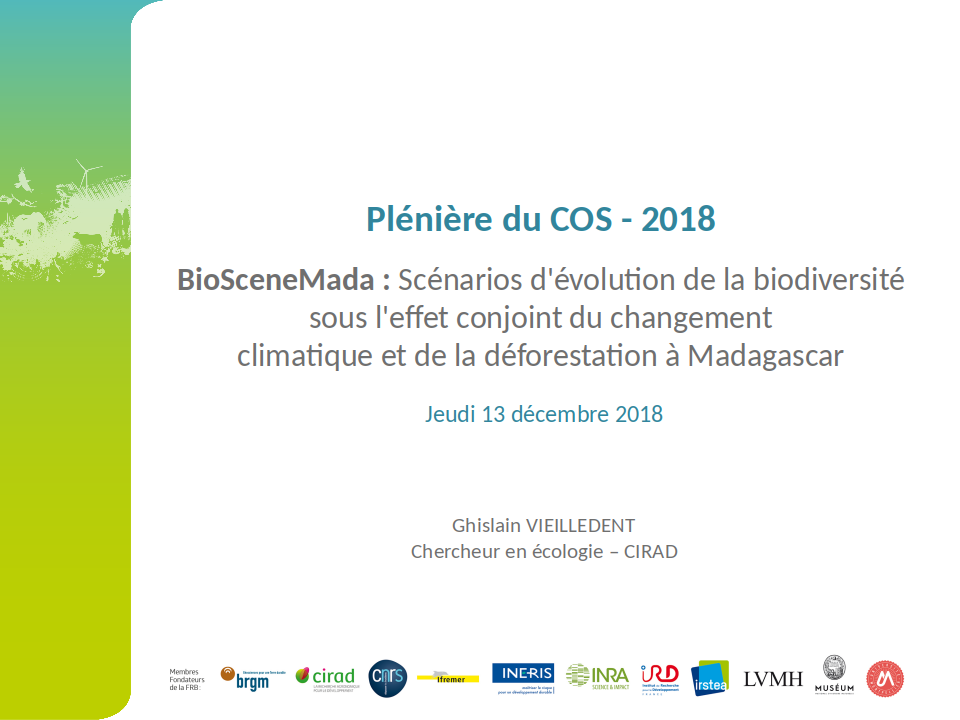
\includegraphics[height=\paperheight,width=\paperwidth]{figs/Masque.png}
%   }
%   \setbeamertemplate{navigation symbols}{}
%   % Remove shadow from block
%   \setbeamertemplate{blocks}[rounded][shadow=false]
%   \begin{frame}[plain]
%   \end{frame}
% }

% Title page
{
  \setbeamertemplate{navigation symbols}{}
  \begin{frame}[plain, noframenumbering]
  \begin{center}
  \small{\textbf{DYAFOR meeting -- March, 1st 2022}}
  \end{center}
  \vspace{-0.5cm}
  \titlepage % Presentation first page
  \vspace{-3cm}
  \begin{center}
    
\includegraphics[width=\textwidth]{figs/Barre_couleur}
    
    \vspace{0.25cm}
    
    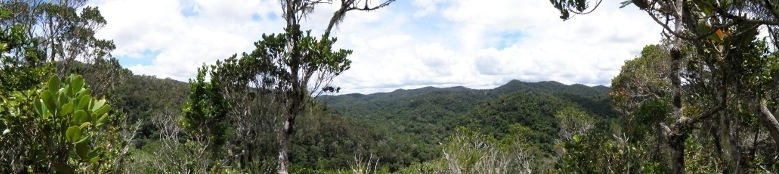
\includegraphics[width=10cm]{figs/Banniere}
    
    \small{Ghislain VIEILLEDENT$^{1, 2}$\hspace{0.25cm}Jeanne CLEMENT$^{1, 2}$\hspace{0.25cm}METRADICA$^{2}$}
      
    \vspace{0.25cm}
    
    {\scriptsize
      \begin{tabular}{l}
        $[1]$ \textbf{Cirad} UMR AMAP, $[2]$ \textbf{METRADICA} Labex CEBA
      \end{tabular}
    }
    
    
\includegraphics[width=0.8\textwidth]{figs/partners_logos}
    
  \end{center}
  \end{frame}
}

% %%%%%%%%%%%%%%%%%%%%%%%%%%%%%%%%%%%%%%%%%%%%%%%%%%%%%%%%%%%%%%%%

\placelogotrue
\begin{frame}
  \frametitle{Plan}
  \begin{columns}[c]
    \begin{column}{0.5\textwidth}
      \tableofcontents[sections=1]
      \vspace{0.5cm}
      \tableofcontents[sections=2]
    \end{column}
    \begin{column}{0.5\textwidth}
        \tableofcontents[sections=3]
        \vspace{0.5cm}
        \tableofcontents[sections=4]
    \end{column}
  \end{columns}
\end{frame}
\placelogofalse

\hypertarget{introduction}{%
\section{Introduction}\label{introduction}}

\hypertarget{jsdms}{%
\subsection{JSDMs}\label{jsdms}}

\begin{frame}{Joint Species Distribution Models (JSDMs)}
\protect\hypertarget{joint-species-distribution-models-jsdms}{}
\textbf{Species Distribution Model (SDM), for one single species.}

\begin{itemize}
\tightlist
\item
  \(y_i \sim Bernoulli(\theta_i)\), \(y_i \in \{0,1\}\)
\item
  \(i\): site
\item
  \(p(\theta_i) = X_i \beta\)
\item
  \(X\): environmental variables
\item
  \(\beta\): species effects
\end{itemize}

\textbf{JSDM \(=\) SDM for community of species.}

\begin{itemize}
\tightlist
\item
  \(p(\theta_{ij}) = \alpha_i + X_i \beta_j + \Sigma_{ij}\)
\item
  \(i\): site, \(j\): species
\item
  Site effect \(\alpha_i\): mean site suitability
\item
  Variance-covariance matrix \(\Sigma_{ij}\): species co-occurrences
\end{itemize}
\end{frame}

\begin{frame}[fragile]{Joint Species Distribution Models}
\protect\hypertarget{joint-species-distribution-models}{}
JSDMs provide a convenient statistical framework to test
\textbf{trait-environment} interactions.

\(\beta_j\) can be expressed as a function of functional traits

\begin{itemize}
\tightlist
\item
  \(p(\theta_{ij}) = \alpha_i + X_i \beta_j + \Sigma_{ij}\)
\item
  \(p(\beta_j) = N(T_j \gamma, V_{\beta})\)
\end{itemize}

JSDMs can help narrow the gap between \textbf{correlative} and
\textbf{mechanistic} species distribution models.

\texttt{jSDM} R package (first chapter of Jeanne's PhD thesis),
\url{https://ecology.ghislainv.fr/jSDM/}
\end{frame}

\hypertarget{metradicas-objectives}{%
\subsection{METRADICA's objectives}\label{metradicas-objectives}}

\begin{frame}{Objectives of METRADICA (Task 3)}
\protect\hypertarget{objectives-of-metradica-task-3}{}
Using JSDMs:

\begin{itemize}
\tightlist
\item
  Test \textbf{trait-environmment} interactions for determining tree
  species distribution in French Guiana.
\item
  Assess species vulnerability to climate change (through contraction of
  species range).
\item
  Interpret species vulnerability to climate change in terms of
  functional traits.
\item
  Derive maps of \(\alpha\) and \(\beta\) diversity for French Guiana.
\item
  Identify refuge area for biodiversity under climate change (stable
  tree communities).
\end{itemize}
\end{frame}

\hypertarget{material-and-methods}{%
\section{Material and methods}\label{material-and-methods}}

\hypertarget{datasets}{%
\subsection{Datasets}\label{datasets}}

\begin{frame}{Datasets}
\protect\hypertarget{datasets-1}{}
\bcols
\bcol{0.5\textwidth}

Three types of data-sets:

\begin{itemize}
\tightlist
\item
  Species occurrences on sites
\item
  Species trait database
\item
  Environmental database
\end{itemize}

\ecol
\bcol{0.5\textwidth}

\centering 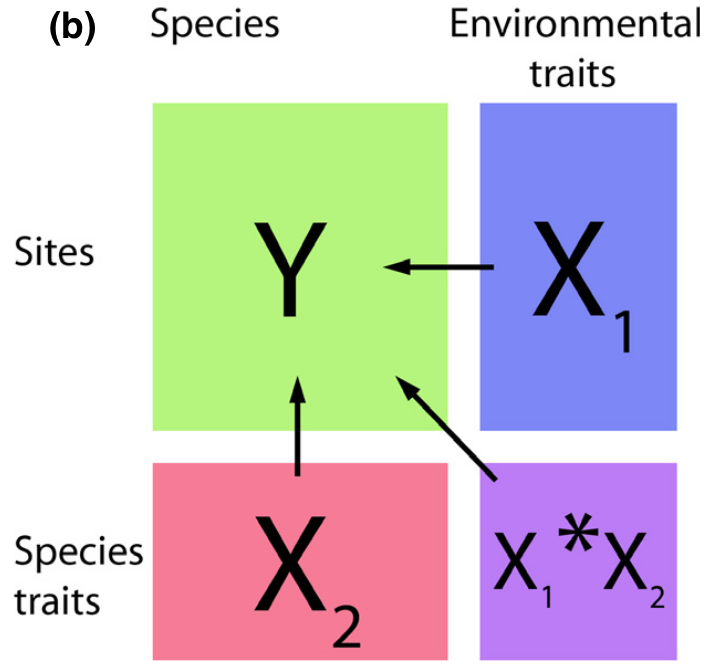
\includegraphics[width=5cm]{figs/four-corner-model} \ecol
\ecols
\end{frame}

\begin{frame}{Occurrences}
\protect\hypertarget{occurrences}{}
\bcols
\bcol{0.5\textwidth}

\begin{itemize}
\tightlist
\item
  Forest plot inventories coming from several networks combined together
\item
  Networks: Guyafor, Gentry, Habitat, Guyadiv
\item
  Presence-absence data and abundances
\item
  285 forest plots
\item
  About 1700 tree species, most of which are rare
\end{itemize}

\ecol
\bcol{0.5\textwidth}

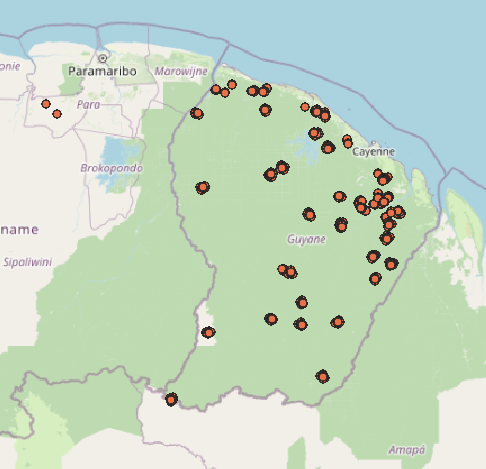
\includegraphics[width=\textwidth]{figs/inventories} \ecol \ecols
\end{frame}

\begin{frame}{Traits}
\protect\hypertarget{traits}{}
\begin{itemize}
\tightlist
\item
  Large ``soft'' trait (WD, LSA, tree max height, etc.) databases from
  previous CEBA projects.
\item
  Five additional mechanistic traits from Metradica project:

  \begin{itemize}
  \tightlist
  \item
    leaf water potential at which cells lose turgor (Ptlp), minimum leaf
    conductance (gmin), leaf saturated water content (LSWC), vein
    density (VLA), stomatal density (SD).
  \item
    24~species, 672 trees, three sites with both hills and valleys
    spread on a precipitation gradient.
  \end{itemize}
\end{itemize}
\end{frame}

\begin{frame}{Environment}
\protect\hypertarget{environment}{}
\begin{itemize}
\tightlist
\item
  Topographic data (SRTM and LiDAR)
\item
  Soil data
\item
  Distance to human infrastructures (roads, villages)
\item
  Climatic data (Chelsa) in the present and the future
\item
  \url{https://guyaclim.cirad.fr}
\end{itemize}
\end{frame}

\hypertarget{study-scales}{%
\subsection{Study scales}\label{study-scales}}

\begin{frame}{Scales: biogeography and micro-environment}
\protect\hypertarget{scales-biogeography-and-micro-environment}{}
\textbf{Local scale: microtopography \(\times\) traits}

\begin{itemize}
\tightlist
\item
  Scale \(=\) \textasciitilde10km, resolution \(=\) \textasciitilde5m
\item
  Explicative model: E \(\times\) T
\item
  Using MNT at 5m: hills (\emph{``terra firme''}) and valleys
\end{itemize}

\textbf{Country scale (French Guiana)}

\begin{itemize}
\tightlist
\item
  Scale \(=\) FG, resolution \(=\) \textasciitilde1km
\item
  Explicative and predictive model
\item
  Two models

  \begin{itemize}
  \tightlist
  \item
    Without traits

    \begin{itemize}
    \tightlist
    \item
      Predictive model
    \item
      Present: distribution and co-occurrences of species
    \item
      Future: range contraction in the future: (i) species vulnerability
      to climate change, (ii) change in species composition
    \end{itemize}
  \item
    With traits

    \begin{itemize}
    \tightlist
    \item
      Explicative model: E \(\times\) T
    \item
      Explaining species location (biogeography)
    \end{itemize}
  \end{itemize}
\end{itemize}
\end{frame}

\hypertarget{perspectives}{%
\section{Perspectives}\label{perspectives}}

\hypertarget{model-comparison}{%
\subsection{Model comparison}\label{model-comparison}}

\begin{frame}{Model comparison with forest dynamics models}
\protect\hypertarget{model-comparison-with-forest-dynamics-models}{}
\textbf{TROLL model}

\begin{itemize}
\tightlist
\item
  Tropical forest dynamics model
\item
  Growth, mortality, recruitment through carbon allocation
\item
  Species parameters are derived from traits
\item
  Calibrated on some forests of French Guiana
\end{itemize}

\textbf{Model comparison}

\begin{itemize}
\tightlist
\item
  Species excluded from the community with TROLL under climate change.
\item
  Do the same species experience a severe range contraction with JSDMs?
\end{itemize}
\end{frame}

\hypertarget{applications}{%
\subsection{Applications}\label{applications}}

\begin{frame}{Applications}
\protect\hypertarget{applications-1}{}
\begin{itemize}
\tightlist
\item
  Anticipating climate change effects on tropical forest in French
  Guiana

  \begin{itemize}
  \tightlist
  \item
    Massive tree mortality events and forest conversion to savannas?
  \item
    Change in species composition?
  \end{itemize}
\item
  Identification of refuge areas for conservation \(\Rightarrow\)
  systematic conservation planning.
\end{itemize}
\end{frame}

% %%%%%%%%%%%%%%%%%%%%%%%%%%%%%%%%%%%%%%%%%%%%%%%%%%%%%%%%%%

{
  % Use background image
  \usebackgroundtemplate{%
    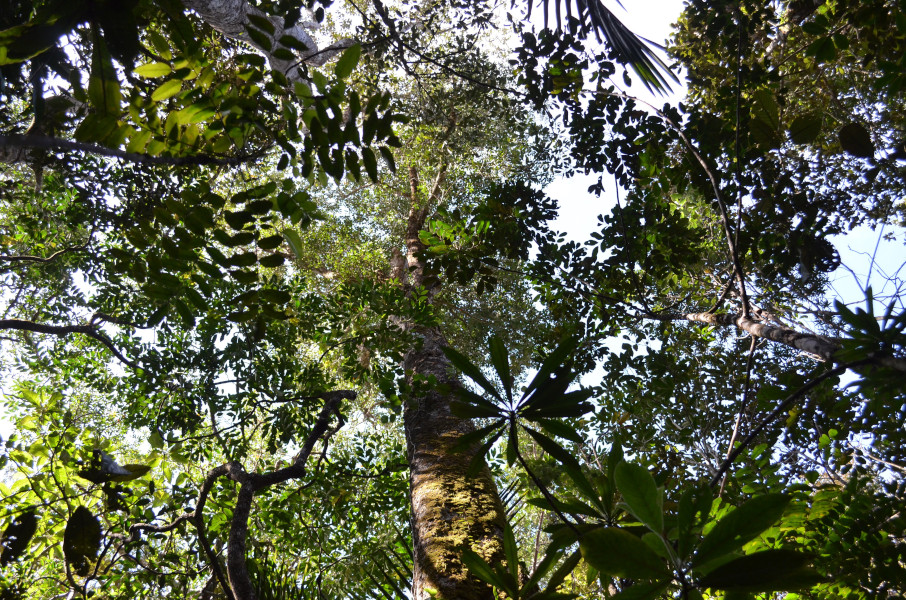
\includegraphics[keepaspectratio=true, height=\paperheight]{figs/Canopy-NC}
  }
  \setbeamertemplate{navigation symbols}{}
  % Remove shadow from block
  \setbeamertemplate{blocks}[rounded][shadow=false]
  \begin{frame}[plain]
  	\vspace*{\stretch{100}} 
    \begin{block}{}
      \begin{center}
        \ldots~Thank you for attention~\ldots \\
        \url{https://ecology.ghislainv.fr/presentations} \\
        
\includegraphics[width=0.8\textwidth]{figs/partners_logos}
      \end{center}
    \end{block}
  \end{frame}
}

\end{document}
